\documentclass[letterpaper,10pt]{article}

\usepackage[english]{babel}
\usepackage[utf8]{inputenc}
\usepackage{amsmath}
\usepackage{graphicx}
\usepackage[colorinlistoftodos]{todonotes}
\usepackage[top=1in, bottom=1in, left=1in, right=1in]{geometry}
\usepackage[small]{titlesec}

\newcommand{\bes}{\begin{equation*}}
\newcommand{\ben}[1]{\begin{equation}\label{#1}}
\newcommand{\ees}{\end{equation*}}
\newcommand{\be}{\begin{equation}}
\newcommand{\ee}{\end{equation}}

\begin{document}

\begin{flushright}
{\Large Josh Bevan - HW 5 Q1 - CS556}
\end{flushright}
\vskip -0.1in
\hrule
\vskip 0.3in

\section*{Does convergence improve or deteriorate as the number of levels increases?}
A problem with $n=2^{10}-1$ was chosen, therefore the coarsest level had $kmax=10$. The problem was solved with varying size V-cycles going to depth $1<kmin<kmax$, for all possible $kmin$. Figure 1 plots the instantaneous convergence factor at iteration 10. As the depth of the V-cycle increases the convergence factor decreases by a moderate amount in this case, from 0.42 to 0.47. This should be unsurprising considering the fewer levels down we go in the V-cycle, the closer the problem directly solved at the coarsest $\mathbf{A}$ is to the original $\mathbf{A}$. Interestingly, the convergence factor is relatively insensitive to the depth of the V-cycle past a certain point; this is convenient in that we are more free to choose an ``optimal'' depth without sacrificing convergence factor (assuming our ``optimal'' depth falls within the insensitive region, which we might expect).

\begin{figure}[!htb]
\centering
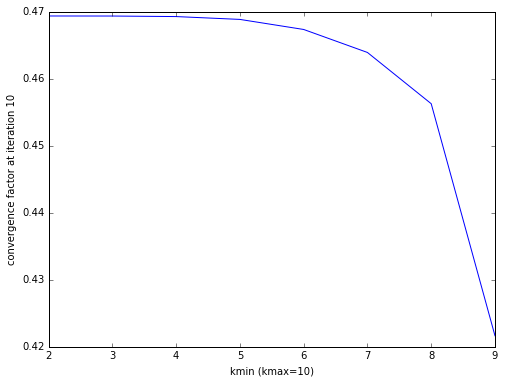
\includegraphics[width=0.6\textwidth]{cnvg.PNG}
\caption{Convergence factor at iteration 10 for various kmin (kmax=10).}
\end{figure}

\section*{Does the cost increase or decrease?}
If we only considered the number of iterations performed for a given depth, then it would appear that a more shallow V-cycle is superior as shown in Figure 2. The residual for the two-level method at a particular iteration will be lower than any of the deeper V-cycles. Of course the cost of the direct solve in the two-level method is likely to be more expensive than going deeper in the V-cycle and a direct solve of a smaller system.

To account for this, each $kmin$'s V-cycle was allowed to iterate for a fixed time rather than fixed number of iterations. If we again plot residual vs iteration number for each, we have the unhelpful Figure 3 plot. Instead it is more useful to plot the time evolution of the residual for each choice of $kmin$, as shown in Figure 4. Here it is much more clear the relative cost of each choice of $kmin$. As the depth of our V-cycle increases the cost per iteration increases, but the cost per equivalent reduction in residual actually decreases (to a point). Given a fixed time budget the two-level method is worse than the three-level method, which in turn is worse than all the deeper V-cycles.

Also important to note is that a $kmin=6$ is actually the lowest time cost per reduction in residual, even better than the deeper V-cycles (lower values of $kmin$). Considering the convergence factor doesn't change much from $kmin=6$ and lower, the relative cost difference is due nearly entirely to the ratio of the cost of a direct solve versus a deeper V-cycle.

\begin{figure}[!htb]
\centering
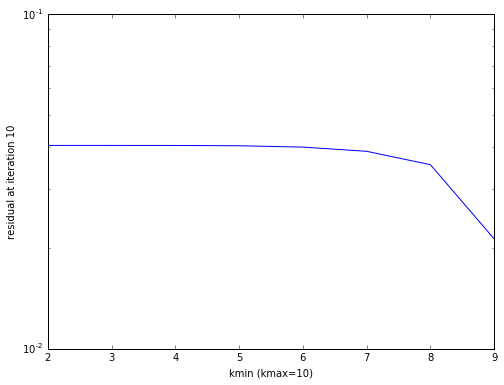
\includegraphics[width=0.8\textwidth]{resit10.PNG}
\caption{Log plot of residual for various kmin (kmax=10) at iteration 10 for all runs.}
\end{figure}

\begin{figure}[!htb]
\centering
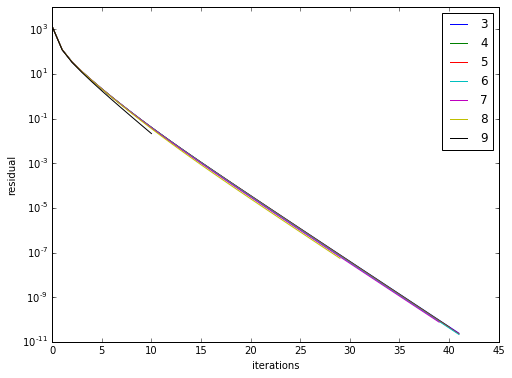
\includegraphics[width=0.8\textwidth]{resit.PNG}
\caption{Log plot of residual for various kmin (kmax=10), all of which have been allowed to run for 60 seconds.}
\end{figure}

\begin{figure}[!htb]
\centering
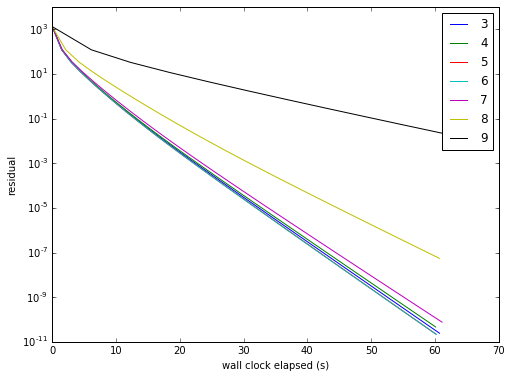
\includegraphics[width=1\textwidth]{restime.PNG}
\caption{Wall clock time evolution of log of residual for various kmin (kmax=10).}
\end{figure}

\end{document}
